\documentclass{article}
\usepackage[brazil]{babel}
\usepackage{graphicx}
\usepackage[utf8]{inputenc}
\usepackage{wrapfig}
\usepackage{geometry}
\usepackage{booktabs}
\usepackage{amsmath}
\usepackage[table,xcdraw]{xcolor}
\usepackage{hyperref}
\usepackage{mathptmx}
\usepackage[T1]{fontenc}
\geometry{verbose,a4paper,tmargin=1.8cm,bmargin=1.8cm,lmargin=1.8cm,rmargin=1.8cm}
\setlength{\parskip}{10pt}	% Vertical distance between two paragraphs
\begin{document}
\begin{titlepage}
\begin{center}
{\large \bf UNIVERSIDADE FEDERAL DO ESP\'IRITO SANTO} \\ 
{\large  Ci\^encia da Computação}\\[5.5cm]
{\large  Rafael Igor Athaydes Rios } \\ [5.5cm]
{\Huge \bf Algoritmos de Ordenação} \\ [12cm]
{Vitória} \\
2015
\end{center}
\end{titlepage}
\newpage
\begin{flushleft}
{\Large \bf{Resumo:}}
\large Este trabalho tem como finalidade apresentar uma disversidade de Algoritmos de Ordena\c{c}\~ao e comparar seus tempos de execução a partir de três tipos diferentes de entrada, são elas: ordenada crescente, decrescente e aleat\'orio.\\
As entradas usadas possuem apenas números inteiros entre 0 e 1.000.000 e tem tamanhos: mil, cinquenta mil, cem mil, quinhentos mil e um milhão.\\
Foram analisados neste trabalho quatorze algoritmos diferentes: bubblesort, shakesort, insertionsort, shellsort, selectionsort, ranksort, quicksort primeiro, quicksort central,
quicksort random, quicksort mediana3, mergesort, heapsort, radixsort e radixbinsort.\\ [1cm]

{\Large \bf Palavras-chave:}
algortimos, ordenação.

\newpage

{\huge \bf Introdução}\\ [1cm]

\hspace{10 mm} Os Algortimos de Ordenação possuem uma grande importância não só na área da computação, mas também no dia a dia. Imagine você ter que consultar seus contatos no telefone sem estarem em ordem alfabética. \\
\hspace{10 mm} Existe uma variedade enorme de algortimos de ordenação conhecidos, cada um com seu tempo de execução. Muitas vezes os algoritmos mais complexos, logo mais difíceis de implementar, são os que possuem os melhores tempos. Mas mesmo assim um algoritmo simples ainda possui utilidade por serem facilmente implementados.

\newpage

{\huge \bf Implementação} \\ [1cm]

\hspace{10mm} Para cada tipo de entrada existe uma tabela e seu respectivo gráfico. O tempo máximo pra cada algoritmo será de 3 minutos (180 s).\\ [1.5cm]

\begin{itemize}
\item \textbf{ Entradas ordenadas crescentes} 

\begin{table}[ht]
\centering
\caption{Entradas Ordenadas Crescentes}
\label{my-label}

\begin{tabular}{l|lllll|}

\cline{2-6}
                                                  &                &           &    \textbf{Tamanhos}& &         \\ \hline
\multicolumn{1}{|c|}{\textbf{Algoritmo}}  & \textbf{1.000     } & \textbf{50.000     } & \textbf{100.000} & \textbf{500.000     } & \textbf{1.000.000      } \\ \hline
\multicolumn{1}{|l|}{Bubblesort} & 0.607          & 10.67           & 42.087           & \textgreater180  & \textgreater180    \\ \hline
\multicolumn{1}{|l|}{Shakesort}           & 0.695          & 0.700           & 0.764            & 1.228            & 1.862              \\ \hline
\multicolumn{1}{|l|}{Insertionsort}       & 0.639          & 0.671           & 0.773            & 1.091            & 1.666              \\ \hline
\multicolumn{1}{|l|}{Shellsort}           & 0.624          & 0.703           & 0.729            & 1.309            & 1.960              \\ \hline
\multicolumn{1}{|l|}{Selectionsort}       & 0.631          & 8.226           & 30.679           & \textgreater180  & \textgreater180    \\ \hline
\multicolumn{1}{|l|}{Ranksort}            & 0.676          & 9.091           & 35.020           & \textgreater180  & \textgreater180    \\ \hline
\multicolumn{1}{|l|}{Quicksort Primeiro}  & 0.662          & 13.130          & 27.763           & 115.584          & \textgreater180    \\ \hline
\multicolumn{1}{|l|}{Quicksort Central}   & 0.697          & 0.699           & 0.718            & 1.179            & 1.882              \\ \hline
\multicolumn{1}{|l|}{Quicksort Random}    & 0.629          & 0.732           & 0.752            & 1.308            & 1.996              \\ \hline
\multicolumn{1}{|l|}{Quick Mediana 3}     & 0.623          & 0.670           & 0.798            & 1.154            & 1.767              \\ \hline
\multicolumn{1}{|l|}{Mergesort}           & 0.628          & 0.689           & 0.759            & 1.303            & 2.152              \\ \hline
\multicolumn{1}{|l|}{Heapsort}            & 0.634          & 0.661           & 0.737            & 1.257            & 2.034              \\ \hline
\multicolumn{1}{|l|}{Radixsort}           & 0.609          & 0.696           & 0.733            & 1.388            & 1.973              \\ \hline
\multicolumn{1}{|l|}{Radixbinsort}        & 0.624          & 0.719           & 0.729            & 1.134            & 1.612              \\ \hline
\end{tabular}
\end{table}

\begin{figure}[!htb]	
   	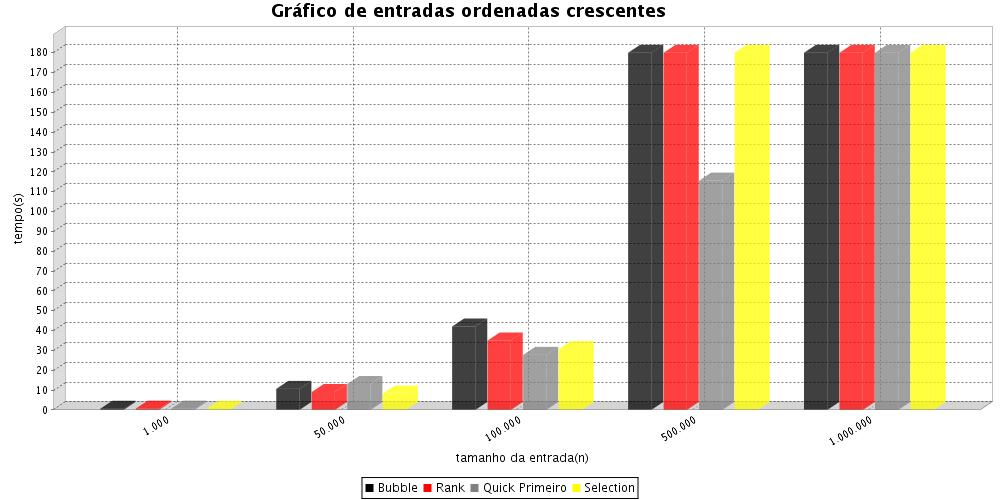
\includegraphics[width=18cm]{grafico1.png}
\end{figure}

\newpage

\begin{figure}[!htb]	
   	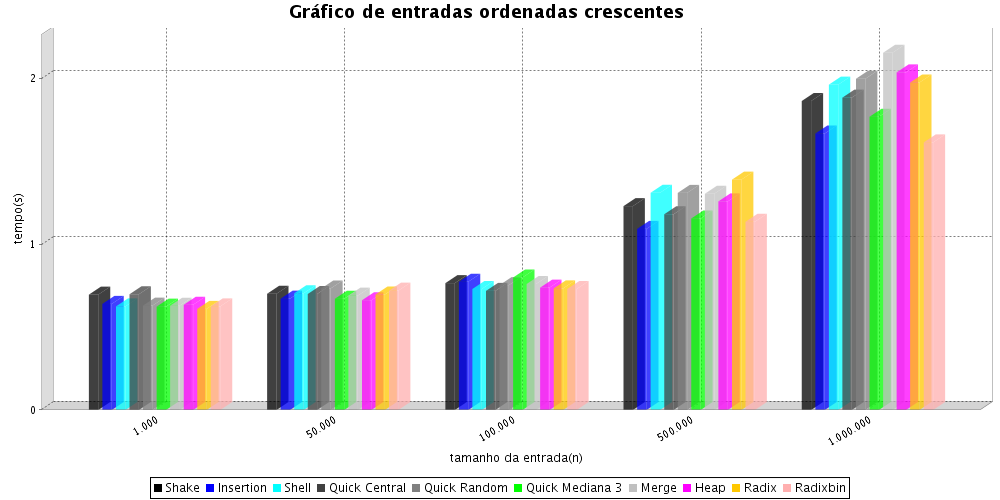
\includegraphics[width=18cm]{grafico2.png}
\end{figure} 
\hspace{10mm} Analizando os resultados percebe-se que os algoritmos bubblesort, selectionsort, ranksort e quickprimeiro possuem o tempo O($n^{2}$), sendo assim, não possuem boa performance com entradas ordenadas crescentes muito grandes, acima de 500 mil números. Com este tipo de entrada o algortimo quick primeiro cai em seu pior caso, onde o pivô é o menor número da entrada, isso faz com que as partições sejam completamente desbalanceadas. \\
\hspace{10mm} Os algortimos shakesort e insertionsort para este tipo de entrada caem no melhor caso, sendo assim eles possuem tempo O(n). \\
\hspace{10mm} Os demais algoritmos conseguem ordenar as entradas com tempos pequenos, o que se já era esperado.
\newpage
\item \textbf{Entradas ordenadas decrescentes}

\begin{table}[ht]
\centering
\caption{Entradas Ordenadas Decrescentes}
\label{my-label}

\begin{tabular}{l|lllll|}

\cline{2-6}
                                                  &                &           &    \textbf{Tamanhos}& &         \\ \hline
\multicolumn{1}{|c|}{\textbf{Algoritmo}} & \textbf{1.000} & \textbf{50.000} & \textbf{100.000} & \textbf{500.000} & \textbf{1.000.000} \\ \hline
\multicolumn{1}{|l|}{Bubblesort}         & 0.578          & 19.644          & 80.902           & \textgreater180  & \textgreater180    \\ \hline
\multicolumn{1}{|l|}{Shakesort}          & 0.662          & 25.934          & 99.455           & \textgreater180  & \textgreater180    \\ \hline
\multicolumn{1}{|l|}{Insertionsort}      & 0.661          & 10.612          & 47.461           & \textgreater180  & \textgreater180    \\ \hline
\multicolumn{1}{|l|}{Shellsort}          & 0.684          & 0.670           & 0.784            & 1.274            & 2.013              \\ \hline
\multicolumn{1}{|l|}{Selectionsort}      & 0.634          & 9.431           & 36.568           & \textgreater180  & \textgreater180    \\ \hline
\multicolumn{1}{|l|}{Ranksort}           & 0.657          & 9.936           & 38.896           & \textgreater180  & \textgreater180    \\ \hline
\multicolumn{1}{|l|}{Quicksort Primeiro} & 0.594          & 8.877           & 18.946           & 97.984           & \textgreater180    \\ \hline
\multicolumn{1}{|l|}{Quicksort Central}  & 0.600          & 0.658           & 0.723            & 1.116            & 1.639              \\ \hline
\multicolumn{1}{|l|}{Quicksort Random}   & 0.593          & 0.647           & 0.716            & 1.270            & 1.930              \\ \hline
\multicolumn{1}{|l|}{Quick Mediana 3}    & 0.614          & 0.659           & 0.737            & 1.191            & 1.719              \\ \hline
\multicolumn{1}{|l|}{Mergesort}          & 0.652          & 0.715           & 0.807            & 1.385            & 2.150              \\ \hline
\multicolumn{1}{|l|}{Heapsort}           & 0.610          & 0.686           & 0.733            & 1.363            & 2.073              \\ \hline
\multicolumn{1}{|l|}{Radixsort}          & 0.612          & 0.732           & 0.941            & 1.750            & 2.666              \\ \hline
\multicolumn{1}{|l|}{Radixbinsort}       & 0.610          & 0.662           & 1.003            & 1.228            & 3.210              \\ \hline
\end{tabular}
\end{table}

\begin{figure}[!htb]	
   	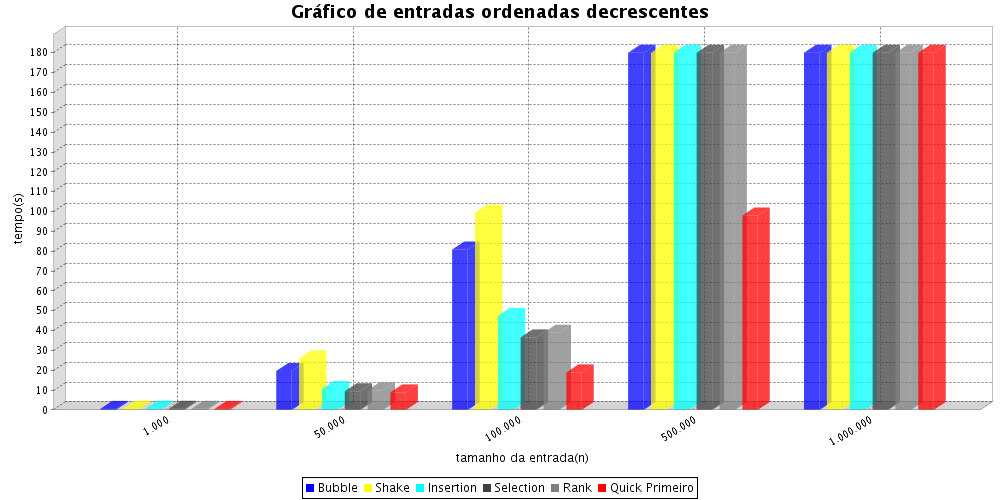
\includegraphics[width=16cm]{grafico3.png}
\end{figure} 
\begin{figure}[!htb]	
   	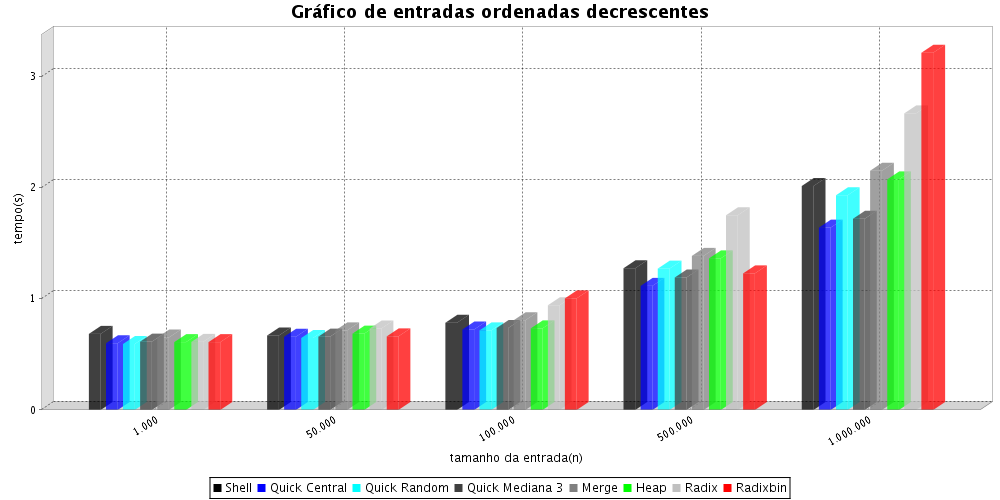
\includegraphics[width=16cm]{grafico4.png}
\end{figure} 

\newpage

\hspace{10mm} Analizando os resultados percebe-se que os algoritmos bubblesort, shakesort, insertionsort, selectionsort, ranksort e quickprimeiro possuem o tempo O($n^{2}$), sendo assim, não possuem boa performance com entradas ordenadas decrescentes muito grandes, acima de 500 mil números. O algoritmo quick primeiro mais uma vez cai em seu pior caso, assim como na entrada crescente, a única diferença é que agora o pivô vai ter o maior número da entrada. \\
\hspace{10mm} Os algoritmos insertionsort e shakesort, que tinham caído no melhor caso para a entrada anterior, neste caso caem no pior caso e passam a ter o tempo O($n^{2}$). \\
\hspace{10mm} Os demais algoritmos continuam com suas performances muito boas. \\ [2cm]

\item \textbf{Entradas aleatórias} \\

\begin{table}[ht]
\centering
\caption{Entradas Ordenadas Decrescentes}
\label{my-label}

\begin{tabular}{l|lllll|}

\cline{2-6}
                                                  &                &           &    \textbf{Tamanhos}& &         \\ \hline
\multicolumn{1}{|c|}{\textbf{Algoritmo}} & \textbf{1.000} & \textbf{50.000} & \textbf{100.000} & \textbf{500.000} & \textbf{1.000.000} \\ \hline
\multicolumn{1}{|l|}{Bubblesort}         & 0.590          & 15.548          & 65.186           & \textgreater180  & \textgreater180    \\ \hline
\multicolumn{1}{|l|}{Shakesort}          & 0.593          & 13.276          & 55.433           & \textgreater180  & \textgreater180    \\ \hline
\multicolumn{1}{|l|}{Insertionsort}      & 0.588          & 4.920           & 18.872           & \textgreater180  & \textgreater180    \\ \hline
\multicolumn{1}{|l|}{Shellsort}          & 0.585          & 0.652           & 0.708            & 1.396            & 2.321              \\ \hline
\multicolumn{1}{|l|}{Selectionsort}      & 0.578          & 7.608           & 34.625           & \textgreater180  & \textgreater180    \\ \hline
\multicolumn{1}{|l|}{Ranksort}           & 0.593          & 10.683          & 47.232           & \textgreater180  & \textgreater180    \\ \hline
\multicolumn{1}{|l|}{Quicksort Primeiro} & 0.574          & 0.636           & 0.703            & 1.214            & 1.815              \\ \hline
\multicolumn{1}{|l|}{Quicksort Central}  & 0.596          & 0.622           & 0.697            & 1.223            & 1.843              \\ \hline
\multicolumn{1}{|l|}{Quicksort Random}   & 0.597          & 0.638           & 0.723            & 1.276            & 1.996              \\ \hline
\multicolumn{1}{|l|}{Quick Mediana 3}    & 0.585          & 0.642           & 0.705            & 1.191            & 1.862              \\ \hline
\multicolumn{1}{|l|}{Mergesort}          & 0.579          & 0.653           & 0.719            & 1.340            & 2.164              \\ \hline
\multicolumn{1}{|l|}{Heapsort}           & 0.580          & 0.644           & 0.721            & 1.377            & 2.427              \\ \hline
\multicolumn{1}{|l|}{Radixsort}          & 0.589          & 0.659           & 0.710            & 1.301            & 1.966              \\ \hline
\multicolumn{1}{|l|}{Radixbinsort}       & 0.585          & 0.621           & 0.666            & 1.080            & 1.939              \\ \hline
\end{tabular}
\end{table}

\begin{figure}[!htb]	
   	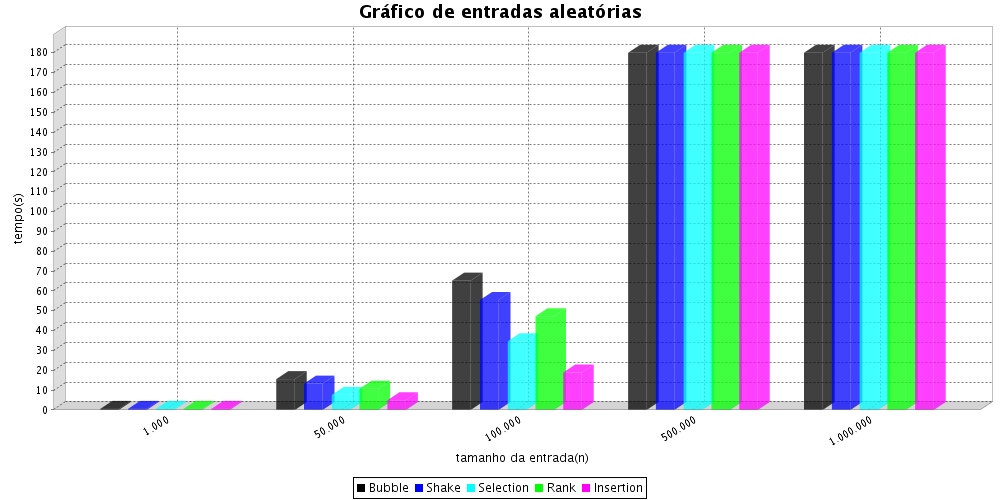
\includegraphics[width=16cm]{grafico5.png}
\end{figure} 
\newpage

\begin{figure}[!htb]	
   	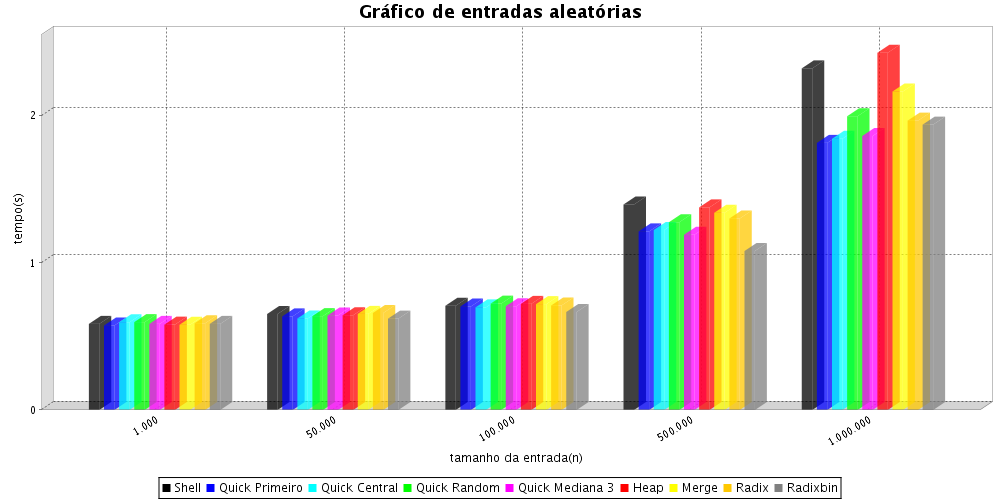
\includegraphics[width=16cm]{grafico6.png}
\end{figure} 

\hspace{10mm} Analizando os resultados percebe-se que os algoritmos bubblesort, shakesort, selction, ranksort e insertionsort possuem as piores performances para entradas acima de 500 mill números, por serem algoritmos O($n^{2}$). O quick primeiro neste tipo de entrada tem tempo O(n $\log n$). \\
\hspace{10mm} Os demais algoritmos possuem performances muito boas, mesmo para entradas muito grandes.
\newpage

\end{itemize}

{\huge \bf Conclusão} \\ [1cm]

\hspace{10 mm} Neste trabalho foi possível verificar a complexidade de 14 algoritmos de ordenação. Percebeu-se que para as entradas ordenada crescente e descrescente o algoritmo Quick Sort Primeiro obteve tempos péssimos, pois caiu em seu pior caso, onde o pivô possui o pior valor possível (maior ou menor da entrada). Para estas mesmas entradas o algoritmo Quick Sort Central possui tempo O(n), pois cai no melhor caso, onde o pivô consegue ser o elemento central. \\
\hspace{10 mm} Em relação aos algoritmos Shake Sort e Insertion Sort, eles obtiveram os melhores resultados na entrada ordenada crescente, isso porque cairam no melhor caso, O(n). No restante eles voltam a ter tempo O($n^{2}$). \\
\hspace{10 mm} Nos algoritmos que conseguiram fazer os testes para todos os tamanhos houve uma vantagem dos algoritmos Quick Sort, mas o Shell Sort merece um grande destaque, pois é simples de entender e facil de implementar.
\end{flushleft}
\end{document}


